\chapter{Models, input data and analysis method}\label{chap:methods}

\section{FLEXDUST}\label{sec:flexdust}
FLEXDUST is an offline global dust emission model developed to be used together 
with FLEXPART to study long-range dust transport and deposition. FLEXDUST relies on common 
formulations for dust emissions found in global climate models \parencite{flexdust_ref_2016}.
FLEXDUST uses a bulk emission scheme as described in \Cref{sec:dust_emission_modelling}.
The version of FLEXDUST used is the latest as of July 17th 2021. 
I modified the FLEXDUST source code slightly to allow the start date, duration and output directory of the simulation to be set dynamically. 
To avoid having to recompile the code each time I changed the starting date of the simulation.  

\subsection{Identification of dust sources}
FLEXDUST identifies the possible dust sources as regions with a high bare soil fraction. 
The bare soil fraction is obtained from the satellite-based Global Land Cover map version 3, by National Mapping Organisations (GLCNMO), with a 
resolution of 15 arcseconds \parencite{shirahata2017production}.
In addition to bare soil regions, FLEXDUST also considers partly vegetated areas as possible
dust sources. The available soil fraction for partly vegetated areas is determined by
subtracting bare soil fraction from the vegetation cover, which is included with the ECWMF meteorological forcing.
FLEXDUST considers depressions to be more favourable to dust emissions as sediments are more easily gathered there \parencite{zender2003mineral}. Therefore FLEXDUST apply the erodibility scaling 
\Cref{eq_ero_soil_frac} according to \textcite{dust_dist_Ginoux2001}. 
\begin{equation}\label{eq_ero_soil_frac}
    S = \left(\frac{z_{max} - z_i}{z_{max} - z_{min}}\right)^5 
\end{equation}    
Here $z_i$ is the local elevation, $z_{max}$ and $z_{min}$ is the minimum and
maximum elevation in a 10\degree $\times$ 10\degree area.  The erodibility $S$ is
then scaled by the bare soil fraction to get the erodible soil fraction. The erodible soil fraction over East Asia is shown in \Cref{fig:erodible_soil_fraction_EA}. 
\begin{figure}[hptb]
    \centering
    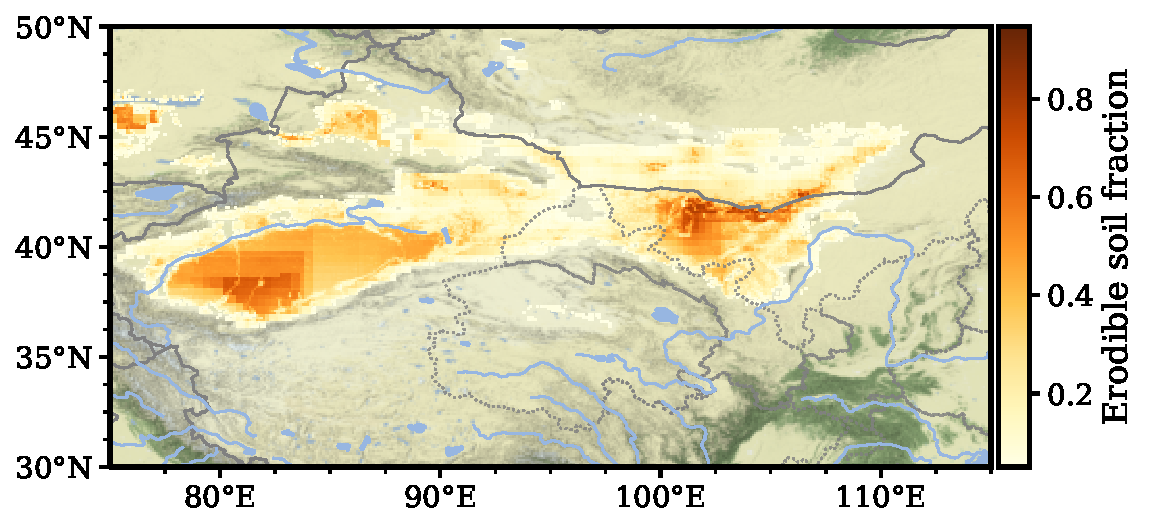
\includegraphics[width=\textwidth]{../figs/erodible_soil_fraction.pdf}
    \caption{The erodible soil fraction from FLEXDUST over the East Asia}
    \label{fig:erodible_soil_fraction_EA}
\end{figure}
\subsection{Dust mobilisation threshold}
The threshold friction velocity follow the idealised expression of \textcite{shao2000simple} in \Cref{eq:treshold_fric_vel}, and is determined by the \SI{75}{\micro\metre} particles. 
For regions with clay and silt present, but no sand, \SI{10}{\micro\metre} 
particles are set to determine the threshold friction velocity. The clay and 
silt fractions can either be obtained from ISRIC 250m resolution Soil Grids dataset 
\parencite{soil-grid_ref}, or using the default Global soil Data \cite{task2014global} dataset. 
The effect of soil moisture on the threshold friction velocity is parametrized according to \textcite{fecan1998parametrization}:
\begin{equation}
    \begin{cases}
    \frac{u_{*tw}}{u_{*t}}=1, & \text{if } w < w' \\
    \frac{u_{*tw}}{u_{*t}}=\sqrt{1+1.21(w-w')^{0.68}}, & w \geq w'
    \end{cases}
\end{equation}
Where $w$ is the volumetric water content of the soil (\%). If the soil moisture exceeds $w'$, the capillary 
forces will start affecting the threshold friction velocity. Here $w'$ is given by \Cref{eq:moisture_clay} 
and depends on the clay content $c$ (\%).   
\begin{equation} \label{eq:moisture_clay}
    w' = 0.17c + 0.0014c^2
\end{equation}
The soil moisture content is retrieved from the ECWMF input fields.
Furthermore, if the surface is covered by snow, dust emissions are assumed to be inhibited. 
Snow cover is available from the ECWMF input fields. 
\par In partly vegetated areas, non-erodible surface elements would increase the surface 
roughness affecting the dust emissions. In FLEXDUST, the drag partition to non-erodible 
surface elements for partly vegetated areas are accounted for following the description in 
\textcite{zender2003mineral}, by scaling the mobilisation threshold by $f_d$ according to \Cref{eq:drag_partition}:
\begin{equation}\label{eq:drag_partition}
    f_d = \left[1 - \frac{\ln (z_{0m}/z_{0s})}{0.35\ln (0.1/z_{0s})^{0.8}}\right]^{-1}
\end{equation}
Here $z_{0m}$ is the roughness length of momentum transfer, and $z_{0s}$ is the smooth roughness length which 
describes the roughness of a bed of potentially erodible particles without any non-erodible elements. Wind tunnel 
experiments have shown that: 
\begin{equation}
    z_{0s} \approx D/30
\end{equation}
where $D$ is the particle diameter. In FLEXDUST it is assumed globally uniform values of  $z_{0m}=\SI{100.0}{\micro\metre}$ and $z_{0s}=\SI{33.3}{\micro\metre}$.

\subsection{Dust flux parameterisation}

After the mobilisation threshold is calculated,  the dust emissions flux is derived following the paremeterisation of the vertical dust flux as described in \textcite{MB95_dust_emission}: 
\begin{equation}
    F=c\alpha \frac{\rho u_{*}^3}{g}\left(1-\frac{u^2_{*t}}{u^2_*}\right)\left(1+ \frac{u_{*t}}{u_*}\right)
\end{equation}
where $u_*$ is the friction velocity, c is a constant scaling factor ($4.8\cdot 10^{-4}$) and $\alpha$ is the sand blasting efficiency:
\begin{equation}\label{eq:sand_blasing_eff}
    \alpha = 100\exp{(13.4f_{clay}-6)\ln 10}
\end{equation}
\Cref{eq:sand_blasing_eff} is only valid for clay fraction $\leq$ 0.2, so if the clay fraction exceed 0.2, it is set to 0.2 \parencite{zender2003mineral}. 


The small dust particles (< \SI{20}{\micro\metre}) has a greater potential to experience long-range transport due to their smaller settling velocities. Since FLEXDUST was developed to study long-range dust transport, the emitted dust is assumed to have a volume size distribution varying between \SI{0.2}{\micro\metre} and \SI{18.2}{\micro\metre}. This size distribution is based on brittle fragmentation theory described in \textcite{kok_scaling_2011}. The log-normal volume size distribution is determined according to \Cref{eq:size_dist}. 

\begin{equation}\label{eq:size_dist}
    \frac{\text{d} V_d}{\text{d} \ln D_d} = \frac{D_d}{c_v}\left[1 + \text{erf}\left(\frac{\ln(D_d/\overline{D_s})}{\sqrt{2}\ln \sigma_s}\right)\right]\text{exp}\left[-\left(\frac{D_d}{\lambda}\right)^3\right]
\end{equation}
Where $c_v = \SI{12.62}{\micro\metre}$ is a normalisation constant, $\overline{D_s}=\SI{3.4}{\micro\metre}$ and $\sigma_s = 3.0$ is the median diameter and the geometric standard deviation respectively.  

\section{FLEXPART}
\par The dust transport and deposition is calculated by the \acrfull{flexpart} \parencite{Flexpart10.4_ref}. FLEXPART is an offline \acrshort{lpdm} that has been applied to study the transport of a wide range of atmospheric tracers, e.g. mineral dust, black carbon and volcanic ash \parencite{flexdust_ref_2016,choi_investigation_2020, eckhardt2008estimation}. 
The version of FLEXPART used is 10.4 and includes the improved wet deposition scheme based on cloud information from the ECWMF input fields \parencite{flexpart_wetdep}. 
\par FLEXPART calculates trajectories for a large number of computational particles (from here on referred to as particles and not be confused with real dust particles) that move according to the wind-fields resolved in the meteorological forcing with parameterizations of the turbulent motions, subgrid-scale convection, and gravitational settling imposed on the trajectories. 
Each particle represents a dust-aerosol population with a log-normal mass size distribution with a specified density and mean particle diameter. 
In addition, ice nucleation efficiency,$IN_{eff}$, cloud condensation nuclei efficiency $CCN_{eff}$ and efficiency of below cloud scavenging by rain $C_{rain}$ and snow $C_{snow}$, can be assigned to the particle regulating the strength of the wet deposition in the model.   

FLEXPART can be either run forward in time from the source to the receptor or backwards from the receptor to the source. The main difference between forward and backward simulations lies in how the emission strength is constrained. 
In a forward simulation, the particles are released at the source. 
The emitted mass which the particles carry is defined before the particle release, directly yielding the concentration and deposition on a regular longitude-latitude grid at each time step.
However, in a backward simulation, the particle release happens at the receptor, and the emission strength is unknown. 
The purpose of the particles in a backward simulation is to probe for the possible source regions and establish the emission sensitivity, i.e. how sensitive the deposition at the receptor would be to a potential source element. 
For more in-depth derivation of source receptor relationships within the framework of \acrshort{lpdm} see Appendix \labelcref{appendix:lpdm_SRR} The final output corresponds to a distribution of possible source areas at each time step.
The emission sensitivity is constructed such that when multiplied by the emission flux with units \si{\kg\per\cubic\metre\per\s} would produce a map of how much each source element is contributing to the concentration or deposition at the receptor.
In a backward simulation, concentration, wet and dry deposition must be obtained through separate simulations as the particle release is set up differently depending on the configuration.  
\subsection{Dry deposition}
In FLEXPART, the dry deposition is represented by a dry deposition velocity $v_d(z)$, and when multiplied with the concentration at a specified height, yields the deposition flux. 
FLEXPART includes both a dry deposition scheme for particulate matter as well as gasses and is calculated based on a two-layer resistance model \parencite{Flexpart-2005_ref_paper}.

In backward mode, dry deposition is calculated at the start of the simulation by releasing the particles in a shallow layer close to the ground. This layer corresponds to the layer in which particles in forward mode would be subjected to dry deposition, and is by default is set to 30m. The "mass" of the particles are then scaled by the deposition velocity and tracked backwards in time as in regular backward simulation \parencite{eckhardt2017source}. 

\subsection{Wet deposition}
The wet deposition scheme in FLEXPART was recently improved in \textcite{flexpart_wetdep} to take advantage of cloud information available from the ECWMF forcing. The wet deposition scheme in FLEXPART consists of two steps.
First, the particle's location in relation to the cloud is determined using the 3D specific \acrfull{ctwc}. Then based on the particle's location in relation to the cloud, the particle can either be subjected to nucleation scavenging inside the cloud or impaction scavenging below the cloud. If the particle is above the cloud, no scavenging can occur. 

In backward mode, the wet deposition is calculated at the time of the particle release. Since wet deposition can occur throughout the whole atmospheric column, the particles are released over the whole atmospheric column to check if any particles are subjected to wet deposition. FLEXPART then calculates the trajectories for wet deposited particles starting at the height where the particles were scavenged, and the remaining particles are terminated.    
\subsubsection{In cloud scavenging}
The in-cloud scavenging scheme in FLEXPART is only activated for particles residing within a precipitating cloud. Precipitation does not necessarily occur over the whole grid cell in the input data. Accordingly, FLEXPART uses an empirical relation to derive the fraction of a gridcell experiencing precipitation; see \textcite{Flexpart-2005_ref_paper} for details. The subgrid precipitating cloud water (PCW) is calculated according to: 
\begin{equation}
    PCW = CTWC\frac{F}{cc}
\end{equation}
Here cc is the surface cloud cover, and F is the precipitating fraction of the gridcell. 

The aerosol scavenging coefficient $\Lambda$ (\si{\per\s}) for in cloud scavenging is given by:
\begin{equation}
    \Lambda = F_{nuc}\left(I/PWC\right)ic_r
\end{equation}
Where $F_{nuc}$ is the nucleation efficiency, I is the precipitation intensity, which is derived from the accumulated precipitation during one time interval in the ECWMF input data, and $ic_r$ is the cloud water replenishment rate. However, $ic_r$ cannot be determined from the ECWMF input data and was determined based on testing in FLEXPART and is considered a tuning parameter in the model.   

In reality, $F_{nuc}$ depends on many different parameters such as aerosol size, chemical composition, temperature and cloud phase. 
A complete parameterization of $F_{nuc}$ in FLEXPART is currently not possible based on the limited information available in the input forcing. 
Still, FLEXPART can account for the fact that aerosols have different nucleation efficiency depending on whether they serve as cloud condensation nuclei (CCN) or ice nuclei (IN). 
% For insoluble aerosols like mineral dust $CCN_{eff}$ primarily depends on the particle size. By itself mineral dust is usually not a very efficient CCN. However, by weathering during transport, the mineral dust aerosols might acquire a coating of some soluble material, e.g. sulphate, increasing its potential to act as a CCN \textcite{Dust_aerosols_coating2001}.     

\subsubsection{Below cloud scavenging}
Dust aerosols residing below the cloud might be scavenged by falling raindrops or snowflakes, called impaction scavenging. 
In FLEXPART, the probability of an aerosol being scavenged by liquid droplets is parameterised according to \textcite{laakso2003ultrafine}. 
The removal of aerosols by falling snowflakes is parameterised in \acrshort{flexpart} according to \textcite{kyro2009snow}.
The efficiency of scavenging by falling rain and snow can be adjusted in the model by changing the $C_{rain}$ and $C_{snow}$ parameter.   

\section{Model input}
\subsection{flex\_extract}
Both FLEXPART and FLEXDUST depend on external meteorological input data. \verb|Flex_extract| is a package developed to retrieve and prepare the necessary meteorological input data from the servers of the \acrfull{ecwmf} \parencite{tipka_flex_extract_2020}. 
\verb|flex_extract| version was 7.0.4 used to retrieve the necessary input fields from the ERA5 reanalysis at a 3hourly temporal resolution and $0.3\degree \times 0.3\degree$ spatial resolution for over the subdomain of East Asia from March until May for the years from 1999 to 2019. 
The retrieval process can be slow, as, in addition to the large amounts of data that needs to be downloaded, the request also has to be processed by the ECWMF servers.


\subsection{ERA5}
ERA5 is the latest reanalysis produced by the ECWMF. 
The ERA5 reanalysis assimilates large amounts of observational data to provide the best estimate of the state of the atmosphere extending back to 1979 \parencite{hersbach_era5_2020}. Compared to its predecessor ERA-Interim, ERA5 offers a higher spatial resolution of $0.25\degree \times 0.25\degree$, up to hourly temporal resolution, and is based on a more recent version of the \acrfull{ifs}. 


\section{Model Setup}\label{sec:Model_setup}

In this thesis, the dust emission model FLEXDUST and the \acrshort{lpdm} FLEXPART was used to 
simulate the springtime dust deposition between 1999 and 2019 at 7 sites across the \acrshort{clp}. 

\textcite{flexdust_ref_2016} used the same two models to study the transport and deposition of high latitude dust, where they simulated the dust transport from a source-oriented viewpoint, following the dust from the source to deposition. 
Here, the dust transport and deposition are simulated from a receptor viewpoint. 
All the dust deposited at the receptor location is tracked backwards in time to probe for possible sources. 
The emission field produced by FLEXDUST then constrains the distribution of possible sources regions. 
The flow chart in \Cref{fig: flow_chart} summarises the modelling workflow. The receptor oriented backward approach was chosen over the forward approach due to being more computationally efficient when the number of source elements greatly exceeds the number of receptors. 
In addition, the backward approach allows for dealing with point receptors naturally \parencite{seibert2004source}. 
% In a forward simulation, the deposition at the receptor location must be interpolated from the model output grid. 
The backward approach also makes it possible to determine exactly the source regions that contribute to deposition at the receptor. 

\begin{figure}[!ht]
  \centering
\begin{tikzpicture}[thick,node distance=2cm, scale=0.6, every node/.style={scale=0.8}]
    \node (start) [startstop, align=center] {\Large \verb|Flex_extract| \\Data retrieval from ECWMF servers};
    \node (in1) [io, below of=start, align=center] {ERA5 input fields \\ 3hourly, \ang{0.3} $\times$ \ang{0.3}};
    \node (flexpart) [process, below right=0.6cm and 0.8cm of in1, align=center] {\Large \verb|FLEXPART| \\ Dust transport and deposition, \\ backward simulations starting from \\ the specified receptor location.};
    \node (flexdust) [process, below left=1cm and 0.8cm of in1, align=center] {\Large \verb|FLEXDUST|};
    \node (emssens_wetdep) [io, below of=flexpart, align=center, xshift=60, node distance=2.5cm] {Wet deposition \\ sensitivity };
    \node (emssens_drydep) [io, below of=flexpart, align=center, xshift=-70, node distance=2.5cm] {Dry deposition \\ sensitivity};
    \node (dust_emissions) [io, below of=flexdust, align=center, node distance=2.9cm] {Dust emission flux \\ \si{\kg\per\square\metre}};
    \node (pprocess) [process, below of=start, align=center, node distance=10cm] {\Large Post processing \\ Emissions sensitivities are multiplied \\ with corresponding dust emissions.};
    \node (source_contrib) [io, below of=pprocess, align=center, node distance=3.5cm, xshift=-50] {\Large Source contribution \\ i.e. how much each source \\ element is contributing to \\ dry and wet deposition at \\ the receptor.};
    \node (stop) [startstop, right of= source_contrib,align=center,  node distance=9cm] {\Large Dust deposition at \\ \Large the receptor \\ the total contribution \\ from all source elements.};
    \draw [arrow] (start) -- (in1);
    \draw [arrow] (in1) -| (flexpart);
    \draw [arrow] (in1) -| (flexdust);
    \draw [arrow] (flexpart) -- (emssens_wetdep);
    \draw [arrow] (flexpart) -- (emssens_drydep);
    \draw [arrow] (flexdust) -- (dust_emissions);
    \draw [arrow] (emssens_wetdep) |- (pprocess);
    \draw [arrow] (dust_emissions) -- (pprocess);
    \draw [arrow] (emssens_drydep) -- (pprocess);
    \draw [arrow] (pprocess) -- (source_contrib);
    \draw [arrow] (source_contrib) -- (stop);
\end{tikzpicture}
\caption{Flow chart showing the workflow for the modelling analysis. }
\label{fig: flow_chart}
\end{figure}

The simulations have been conducted on the Saga high performance computing cluster operated by the Norwegian high performance 
computing centre, Sigma2. For storage and post-analysis, the data is transferred to the 
\acrfull{nird} computing infrastructure. 

FLEXPART and FLEXDUST were run at a 3hourly temporal resolution, with $0.1\degree \times 0.1\degree$ output grid and driven by  ERA5 meteorological forcing data. 
% FLEXDUST was set up at the same temporal and output grid as FLEXPART.  
As described in \Cref{chap:east_asia_dust} dust events are primarily occurring in spring. 
Therefore, I only simulated the spring months from March until May.  I ran the models over a 20 year period to provide insight on the inter-annual variation in the dust source regions to the \acrshort{clp}.   
\subsection{FLEXPART}
To make it possible to multiply the emission sensitivity with the dust emission flux, FLEXPART has to be set up such that each particle release is kept separate in the output. 
Therefore, I  specified a new particle release in the \verb|RELEASES| file for each forward time step. I limited the length of the trajectory to five days by specifying a time limit in the \verb|NAGECLASSES| file.
The FLEXPART output file then contains two temporal dimensions, one \verb|time| dimension going from the last date backwards to the start date of the simulation and the \verb|pointspec| dimension representing each release. 
To allow for all the backward trajectories to complete, I let the last release happen five days after the starting date of the simulation.   
The particle release is specified at 3rd hourly intervals. The number of particles released in each release is 50000 particles and 200000 particles for dry and wet deposition simulations respectively. 
More particles are needed in the wet deposition simulation to achieve statically robust results due to how the particle release is set up.  
A copy of the exact FLEXPART and FLEXDUST source code used can be accessed at \url{10.5281/zenodo.5128338}. 
\begin{figure}[htpb]
    \centering
    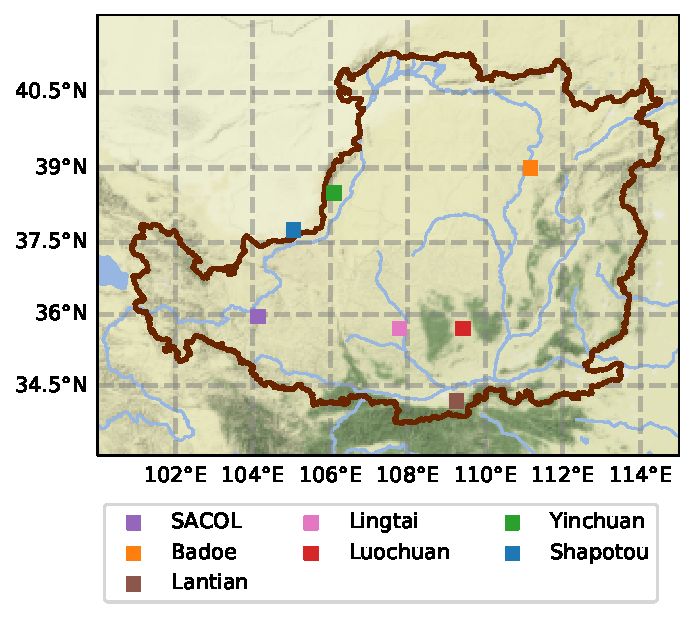
\includegraphics[width=0.7\textwidth]{texfiles/figs/map_loess.pdf}
    \caption{Map of the receptor points, specified in the FLEXPART simulations}
    \label{fig:maps_clp_location}
\end{figure}

To provide insight on the spatial variation in the dust source contribution to the \acrshort{clp}, seven well known Loess sites distributed across the \acrshort{clp} were selected as receptor points in FLEXPART  (\Cref{fig:maps_clp_location}), namely: SACOL, Shapotou and Yinchuan in the north-west, Lingtai, Luochuan and Lantian in the south-east and Badoe in the north-east. 
The exact coordinates of the receptor locations are listed in \Cref{tab:coordinates_clp}. 



Moreover, two particles size bins, \SI{1.7}{\micro\metre}-\SI{2.5}{\micro\metre} representing clay particles and  \SI{15}{\micro\metre}-\SI{20}{\micro\metre} size bin representing silt sized particles were included in the FLEXPART simulations . 
The two particle size bins do not only differ in size, but they also have different assumptions on the $CCN_{eff}$. 
The parameters for the two particle species are listed in \Cref{tab:particle_params}. 
I included only two size bins as a trade-off to allow running multiple years and keep the computational demand reasonable.  
 
\begin{table}[htpb]
\caption{FLEXPART species parameters for "clay" and "silt" particle size bin}
\label{tab:particle_params}'
\centering
% \resizebox{\textwidth}{!}{%
\begin{tabular}{@{}lll@{}}
\toprule
 & Clay  & Silt \\ \midrule
\verb|PCRAIN_AERO| & 1.00  & 1.00 \\
\verb|PCSNOW_AERO| & 1.00  &  1.00 \\
\verb|PCC_AERO| & 0.45 \parencite{flexdust_ref_2016}   &  0.90\parencite{flexdust_ref_2016} \\
\verb|PIN_AERO| & 0.10 \parencite{flexdust_ref_2016} & 0.10 \parencite{flexdust_ref_2016} \\
\verb|PDENSITY| & \SI{2500.0}{\kg\per\cubic\metre}    & \SI{2500.0}{\kg\per\cubic\metre} \\
\verb|PDQUER| & \SI{2.057E-6}{\metre}    &  \SI{17.32E-6}{\metre}   \\
\verb|PDSIGMA| & 1.21   &  1.15    \\ \bottomrule
\end{tabular}%
% }
\end{table}
 
Given that all the FLEXPART simulations are independent of each other, it was easy to take advantage of the parallel computing capabilities of Saga. By splitting the simulation into several independent FLEXPART simulations, each covering one month, the simulation could be run across multiple CPUs simultaneously.
All in all, this added up to a total of 1680 individual FLEXPART simulations.
To help set up all the FLEXPART simulations, a python script\footnote{https://github.com/Ovewh/FLEXPART-script} was developed. 

\subsection{FLEXDUST}
Compared to \acrshort{flexpart}, FLEXDUST is much less demanding to run. The FLEXDUST simulation was split into sub simulations covering one spring, and the whole simulation took a few hours to complete on the supercomputer. 
The soil texture dataset used was the ISRIC 250m Soil grids dataset. The ISRIC dataset was proven based on model sensitivity experiments to represent better East Asian dust sources than the default soil texture dataset.      

\subsection{Model validation}\label{sec:model_eval_discription}
There are very few measurements of dust deposition fluxes that separate both dry and wet deposition and had a sufficient temporal resolution to evaluate the performance of FLEXPART/FLEXDUST. \textcite{osada2014wet} published a data set of monthly dry and wet deposition fluxes from 6 locations by the coast of Japan, providing measurement from November 2008 until December 2010. They used a 4-stage filtration approach to separate the deposited dust into four size bins  >\SI{20}{\micro\metre}, \SI{20}{\micro\metre}-\SI{10}{\micro\metre}, \SI{10}{\micro\metre}-\SI{5}{\micro\metre} and \SI{5}{\micro\metre}-\SI{1}{\micro\metre}. 
The four particle size bins were simulated separately in FLEXPART and were assumed to follow the same size distribution as in the main model experiment. The Hedo, Fukuoka, Tottori and Toyama sites were used as receptor points in FLEXPART. 

\begin{figure}[htpb]
    \centering
    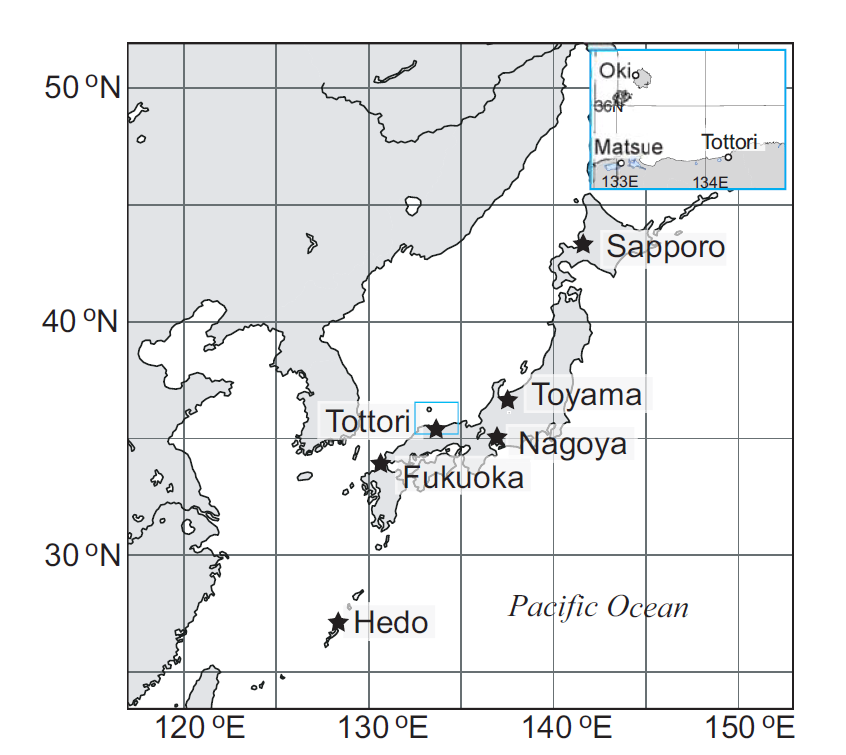
\includegraphics[scale=0.45]{texfiles/figs/Osada_locations.PNG}
    \caption{Map of the locations where dust deposition where sampled \parencite{osada2014wet}}
    \label{fig:map_japan}
\end{figure}



\subsection{Model sensitivity experiments}
Sensitivity experiments are a crucial part of any modelling study. A model sensitivity analysis aims to quantify the impact of possible errors and differences in the input data on the predicted model output. Four sensitivity experiments were conducted to investigate the impact of (1) different forcing data, (2) varying particle density, (3) choice of soil texture data and (4) and below cloud scavenging. All the sensitivity experiments were done for 2019 except the forcing experiment done for 2015. Except for the parameters listed in \Cref{tab:sensitivity_exp} all other parameters are equal to the main model experiment described previously. 

% The reason for testing the model with different forcing data is to examine how sensitive the results are to the choice of input data. The two forcing dataset compared in the sensitivity analysis is the latest generation of \acrshort{ecwmf} reanalysis, ERA5 against the previous generation of reanalysis ERA-Interim. This analysis would allow to whether using a the new higher resolution ERA5 as input data improves the representation of dust in the models. Moreover, if the difference between the two forcing dataset can reasonably explain based on there known differences, it means that  
\begin{table}[htpb]\label{tab:sensitivity_exp}
\caption{The model sensitivity experiments that have been performed}
\centering

\resizebox{\textwidth}{!}{%
\begin{tabular}{@{}lllll@{}}
\toprule
 Sensitivity experiment & Soil map  & Forcing & Below cloud scavenging & Particle density \\ \midrule
 Model forcing & ISRIC  & ERA-Interim & Yes & \SI{2500}{\kg\per\cubic\cm}  \\
 Particle density & ISRIC & ERA5  & Yes & \SI{2200}{\kg\per\cubic\cm}-\SI{2800}{\kg\per\cubic\cm}  \\
 Soil texture & Default & ERA5 & Yes & \SI{2500}{\kg\per\cubic\cm}   \\
 Cloud scavenging& ISRIC  & ERA5 & No & \SI{2500}{\kg\per\cubic\cm} \\ \bottomrule

\end{tabular}%
}
\end{table}



\section{Analysis Tools}

The analysis and post-processing of the model output are achieved using a handful of python libraries. More details on the specific software used and developed to facilitate the analysis are provided in Appendix \labelcref{appendix:software}.
\subsection{Post-processing of model output}
The FLEXDUST emission flux has to be matched with the corresponding emission sensitivity to calculate the source contribution and deposition at the receptor. 
However, there is currently no software available that can match output from a backward simulation with an emission inventory. 
Therefore considerable effort had to be spent towards developing a code that could combine the FLEXPART and FLEXDUST output.   
This was achieved by first reshaping the FLEXPART output data to a format that would easily match with FLEXDUST. 
Therefore, a new backwards time dimension with a length equal to maximum particle age (in this case, 5 days) was created and the 
 \verb|pointspec| dimension was set as the forward time dimension. 
This format proved to be a more efficient way of storing the output from these kinds of backward simulations since the raw output format would only contain zeros after the maximum age was exceeded. When the output was converted to the new format, it was straightforward to match the FLEXDUST emission inventories with the FLEXPART emission sensitivity. 

 After the FLEXPART and FLEXDUST output have been combined final step is to scale the source contribution by the fraction of the size distribution corresponding to the specific size bin listed in \Cref{tab:size_distribution}. The assumed size distribution in \Cref{tab:size_distribution} is the same size distribution used in FLEXDUST to generate RELEASE files for forward FLEXPART simulation and follow the log-normal distribution of \Cref{eq:size_dist}.  


\begin{table}[htpb]
    \caption{Assumed size distribution of emitted dust in FLEXPDUST}
    \label{tab:size_distribution}
    \centering
    \begin{tabular}{@{}ll@{}} 
    \toprule
        bin width (\si{\micro\metre}) &  fraction \\ \midrule
         0.02 –  0.1 & 0.0030\\
         0.1 – 0.5 &  0.0163\\
         0.5 - 1.0 &0.0327\\
         1.0 – 1.7 & 0.0556\\
         1.7 – 2.5 & 0.0820\\
         2.5 – 5.0 &  0.1605\\
         5.0 – 7.5 & 0.2209\\
         7.5 – 10 & 0.2425\\
         10 – 15 & 0.1516 \\
         15 – 20 & 0.0349 
    \end{tabular}

\end{table}

\subsubsection{Snakemake workflow}
To manage the considerable amount of data produced by \acrshort{flexpart}, a \verb|snakemake| workflow was implemented.   
\verb|Snakemake| is a workflow management system \parencite{molder2021sustainable} that can keep track of all dependencies and steps required to generate a specific result.
This means that any changes made to a file at the beginning of the workflow \verb|snakemake| would notice and regenerate all the results depending on that file. 
\verb|Snakemake| also keeps track of which steps of the analysis have been completed, so if anything happened while the analysis is running, it does not have to from the beginning. 
\verb|Snakemake| works by defining a sequence of rules that takes predefined input files based on a specified filename pattern. 
Based on this filename pattern \verb|snakemake| knows which rules to run that generates the desired output file. \Cref{fig:rule_graph_eks} show an example of how this sequence of rules might look like.  
 \begin{figure}[htpb]
     \centering
     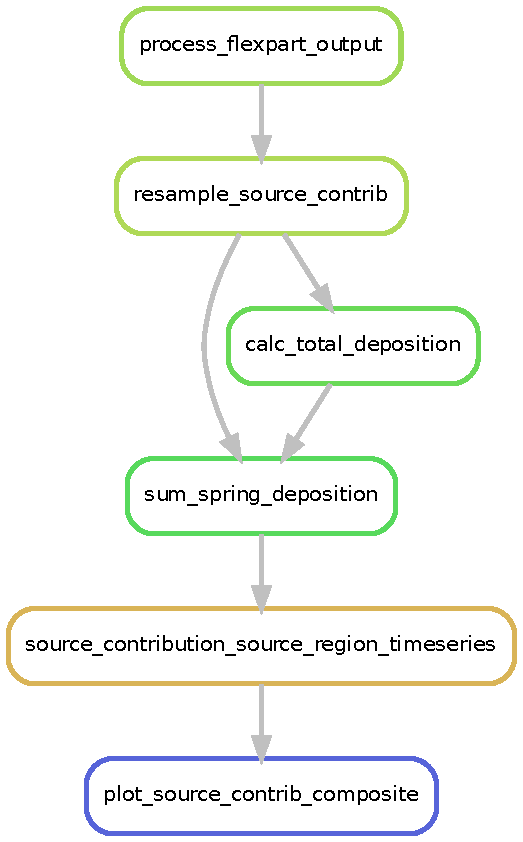
\includegraphics[width=0.4\textwidth]{texfiles/figs/rulegraph_eks.pdf}
     \caption{Example rulegraph for generating \Cref{fig:source_contrib2mmu_anomalies} and \Cref{fig:source_contrib20mmu_anomalies}}
     \label{fig:rule_graph_eks}
 \end{figure}  

\subsection{FLEXPART trajectory analysis}\label{chap:method_trajec_analysis}
In addition to emission sensitivity, FLEXPART can also output information about particle trajectories. Including calculating the centroid trajectory and cluster trajectories of the particle cloud. 
Unfortunately, the clusters produced by FLEXPART are not very informative, as the clustering routine only considers the position of the particles at the output time and does not consider which cluster it was previously assigned to. However, the centroid trajectory can still provide insight into the dust transport paths. 
The original idea was to take the centroid trajectories of every particle release and then cluster the centroid trajectories to obtain a set of trajectories representing the main dust transport pathways. 
This procedure is described in more detail in Appendix \labelcref{chap:trajec_analysis}. However, this did not work out for two reasons, (1) it was challenging to define a suitable distance metric, and (2) the centroid trajectories is an average of both dust loading and non-dust loading trajectories, thus smoothing out the dust transport paths. 
Therefore making a clever selection and averaging of the trajectories proved to be more informative. 

% The optimal approach would be do clustering based on the particle position, however this was not infeasible do here since the amount of data would become too much. Analysing the particle positions is better suited for case studies of transport during of single dust storms.       
The current trajectory analysis was done by first filtering out the  non-dust centroid trajectories, based on whether dust was deposited at the receptor at the time of arrival. Then all the dust loading trajectories were given a weight based on their dust loading and averaged to make one weighted average centroid trajectory. This averaged centroid dust loading was then applied to diagnose the dust transport path sways to the receptor points.       
 

\subsection{Composite analysis}

A composite analysis is a useful method for identifying climatic features that are difficult to observe in its totally. 
A composite analysis involves collecting several cases of a given situation, e.g. years with strong deposition, and create an average representation of meteorological conditions in that given situation, e.g. surface winds during strong deposition years. 
The change can then be enlarged further by subtracting the weak composite from the strong composite to show the composite anomalies. 
     
\subsection{Empirical orthogonal function}

\acrfull{eof} analysis is often used in climate studies to identify the regions with the largest variability and study how they change with time. 
The \acrshort{ao} is an example of a climatic feature that was first described based on an \acrshort{eof} analysis \parencite{thompson1998arctic}. Here the \acrshort{eof} analysis was done using \verb|eofs| python package \parencite{dawson2016eofs}.  

-